\documentclass[aspectratio=169,10pt]{beamer}

\usetheme{Madrid}
\usecolortheme{default}

\usepackage{amsmath,amssymb}
\usepackage{booktabs}
\usepackage{microtype}
\usepackage{xcolor}
\usepackage{graphicx}

\graphicspath{{figures/}}

% Professional Academic Theme Styling (NITK Surathkal Palette)
\definecolor{nitkblue}{RGB}{18,52,102}
\definecolor{nitkgold}{RGB}{212,160,23}
\definecolor{muted}{RGB}{95,105,120}
\definecolor{warnred}{RGB}{185,45,35}
\definecolor{goodgreen}{RGB}{40,135,65}

\setbeamercolor{palette primary}{bg=nitkblue,fg=white}
\setbeamercolor{palette secondary}{bg=nitkblue!85,fg=white}
\setbeamercolor{palette tertiary}{bg=nitkblue!70,fg=white}
\setbeamercolor{structure}{fg=nitkblue}
\setbeamercolor{title}{bg=nitkblue,fg=white}
\setbeamercolor{titlelike}{bg=nitkblue,fg=white}
\setbeamercolor{block title}{bg=nitkblue,fg=white}
\setbeamercolor{block body}{bg=nitkblue!6,fg=black}
\setbeamercolor{block title alerted}{bg=warnred,fg=white}
\setbeamercolor{block body alerted}{bg=warnred!6,fg=black}
\setbeamercolor{block title example}{bg=goodgreen,fg=white}
\setbeamercolor{block body example}{bg=goodgreen!6,fg=black}

\setbeamertemplate{navigation symbols}{}
\setbeamertemplate{footline}[frame number]
\setbeamertemplate{blocks}[rounded][shadow=false]
\setbeamertemplate{itemize item}[circle]
\setbeamertemplate{itemize subitem}[triangle]

\title[MATP Unified Monorepo]{MATP: Memory-Augmented Tool Policy for Long-Horizon Autonomous Agents}
\subtitle{Causal State Invalidation $\cdot$ Temporal Decay $\cdot$ Hierarchical Macro Distillation $\cdot$ Tool Policy Learning}
\author[Saravanan, Hegde, Muhammed]{Rahul Saravanan \and Shishir Hegde \and Ashab Muhammed}
\institute[NITK Surathkal]{
  Department of Information Technology \\
  National Institute of Technology Karnataka, Surathkal \\
  \vspace{0.3em}
  \textit{7th Semester Major Academic Project (MATP)}
}
\date{November 2026}

\begin{document}

% -----------------------------------------------------------------------------
% SLIDE 1: Title Slide
% -----------------------------------------------------------------------------
\begin{frame}[plain]
  \vfill
  \centering
  \begin{beamercolorbox}[sep=10pt,center,rounded=true,shadow=false,wd=0.96\linewidth]{title}
    {\usebeamerfont{title}\Large \textbf{MATP: Memory-Augmented Tool Policy}}\par
    \vspace{0.4em}
    {\usebeamerfont{subtitle}\normalsize \textbf{A Unified Framework for Long-Horizon Autonomous Agents}}\par
    \vspace{0.2em}
    {\scriptsize Causal State Invalidation $\cdot$ Temporal Decay $\cdot$ Macro Distillation $\cdot$ Policy Learning}
  \end{beamercolorbox}
  
  \vspace{1.2em}
  {\normalsize \textbf{Rahul Saravanan \quad $\cdot$ \quad Shishir Hegde \quad $\cdot$ \quad Ashab Muhammed}}\par
  \vspace{0.6em}
  {\small \textbf{Department of Information Technology} \\ \textbf{National Institute of Technology Karnataka (NITK), Surathkal}}\par
  \vspace{0.6em}
  {\scriptsize \textit{7th Semester Capstone Project Defense $\cdot$ November 2026}}\par
  \vfill
\end{frame}

% -----------------------------------------------------------------------------
% SLIDE 2: The Core Problem in Long-Horizon Agentic Systems
% -----------------------------------------------------------------------------
\begin{frame}{The Long-Horizon Problem: Why Standard Agents Fail}
  \begin{columns}[T,onlytextwidth]
    \begin{column}{0.48\textwidth}
      \begin{block}{1. The FIFO Context Trap}
        \begin{itemize}
          \item Context pruning evicts early steps first.
          \item Foundational invariants (schemas, secrets) are lost.
          \item \textbf{Impact:} 75\% critical early state forgotten over 40 steps.
        \end{itemize}
      \end{block}
      \vspace{0.3em}
      \begin{block}{2. The Naive RAG Trap}
        \begin{itemize}
          \item Unversioned vector search indexes mutating files.
          \item Semantic similarity contains no concept of invalidation.
          \item \textbf{Impact:} 40\% stale-state leakage (superseded schemas float up).
        \end{itemize}
      \end{block}
    \end{column}

    \begin{column}{0.48\textwidth}
      \begin{alertblock}{3. Procedural Thrashing \& Schema Errors}
        \begin{itemize}
          \item Static system prompts lack dynamic empirical feedback.
          \item Agents get trapped in repetitive trial-and-error tool loops.
          \item Syntax errors (e.g. SQLite syntax quirks) repeat endlessly.
        \end{itemize}
      \end{alertblock}
      \vspace{0.3em}
      \begin{exampleblock}{The MATP Monorepo Solution}
        A unified local MCP system combining:
        \begin{itemize}
          \item \textbf{Causal DAG} state tracking ($W_{\text{DAG}}$).
          \item \textbf{Temporal decay} \& adaptive $\lambda$ learning.
          \item \textbf{Macro distillation} \& self-healing policies.
        \end{itemize}
      \end{exampleblock}
    \end{column}
  \end{columns}
\end{frame}

% -----------------------------------------------------------------------------
% SLIDE 3: Unified Monorepo Architecture (Wide Horizontal View)
% -----------------------------------------------------------------------------
\begin{frame}{Unified System Architecture: End-to-End Pipeline}
  \centering
  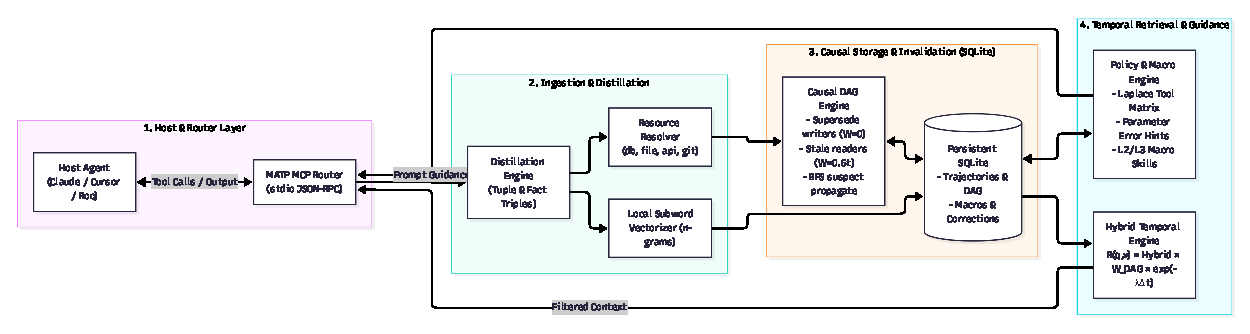
\includegraphics[width=\textwidth,height=0.48\textheight,keepaspectratio]{architecture_horizontal.pdf}
  \vspace{0.4em}
  \begin{columns}[T,onlytextwidth]
    \begin{column}{0.32\textwidth}
      \begin{block}{\footnotesize 1. Ingest \& Distillation}
        \scriptsize Distills raw tool outputs into structured tuples; extracts canonical resources. $13.5\times$ compression.
      \end{block}
    \end{column}
    \begin{column}{0.32\textwidth}
      \begin{block}{\footnotesize 2. Causal Storage (SQLite)}
        \scriptsize Tracks resource versions, supersedes older writers, marks readers stale, propagates taint via DAG.
      \end{block}
    \end{column}
    \begin{column}{0.32\textwidth}
      \begin{block}{\footnotesize 3. Retrieval \& Policy}
        \scriptsize Hybrid scoring with exponential decay $e^{-\lambda \Delta t}$, Laplace candidate matrix, auto-correction hints.
      \end{block}
    \end{column}
  \end{columns}
\end{frame}

% -----------------------------------------------------------------------------
% SLIDE 4: Contribution 1: Temporal & State-Aware Versioning
% -----------------------------------------------------------------------------
\begin{frame}{Contribution 1: Versioning with Piecewise Temporal Scoring}
  \begin{block}{Piecewise Retrieval Formula $R(q, v_i)$}
    \vspace{-0.2em}
    \begin{equation*}
      R(q, v_i) = 
      \begin{cases}
        0, & \text{if } v_i \text{ is superseded or depends on invalid state}, \\
        S(q, v_i) \cdot W_{\text{DAG}}(v_i) \cdot e^{-\lambda(t_{\text{curr}} - t_i)}, & \text{otherwise}.
      \end{cases}
    \end{equation*}
  \end{block}

  \begin{columns}[T,onlytextwidth]
    \begin{column}{0.48\textwidth}
      \begin{block}{Causal Logical Clock $t$}
        \begin{itemize}
          \item Discrete causality steps, not noisy wall-clock time.
          \item Explicit version tracking across resources.
          \item Hard zeroing prevents obsolete state leakage.
        \end{itemize}
      \end{block}
    \end{column}

    \begin{column}{0.48\textwidth}
      \begin{block}{Online Adaptive Decay Calibration}
        \begin{equation*}
          \lambda_{\text{task}} \leftarrow (1-\eta)\lambda_{\text{task}} + \eta \frac{\ln 2}{\text{median}(\Delta t_{\text{useful}})}
        \end{equation*}
        \begin{itemize}
          \item Learns optimal half-life per task from feedback.
          \item Rapid debugging $\to$ large $\lambda$; refactoring $\to$ small $\lambda$.
        \end{itemize}
      \end{block}
    \end{column}
  \end{columns}
\end{frame}

% -----------------------------------------------------------------------------
% SLIDE 5: Contribution 2: Causal State Invalidation (Wide Flowchart)
% -----------------------------------------------------------------------------
\begin{frame}{Contribution 2: Causal State Invalidation \& Provenance Tracking}
  \centering
  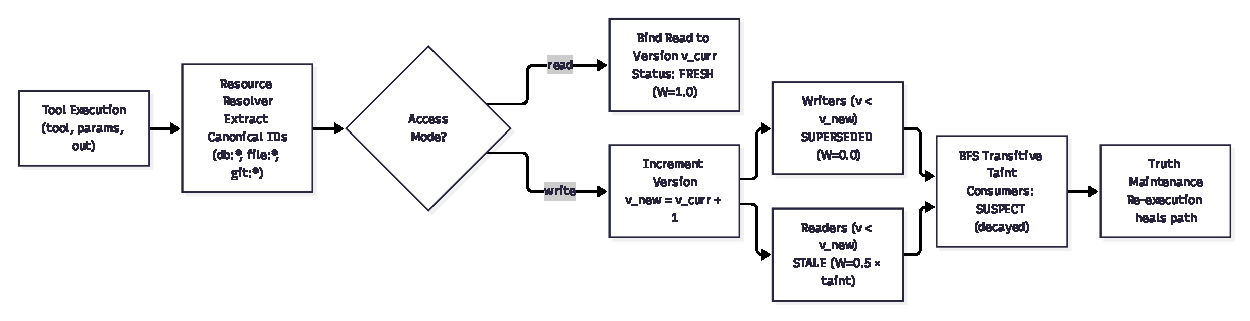
\includegraphics[width=0.98\textwidth,height=0.46\textheight,keepaspectratio]{dag_flowchart_horizontal.pdf}
  \vspace{0.4em}
  \begin{columns}[T,onlytextwidth]
    \begin{column}{0.32\textwidth}
      \begin{block}{\footnotesize Direct Supersession ($W=0$)}
        \scriptsize Newer write $v_{new}$ supersedes older writers of the same resource immediately ($W=0.0$).
      \end{block}
    \end{column}
    \begin{column}{0.32\textwidth}
      \begin{alertblock}{\footnotesize Reader Staleness ($W=0.5\tau$)}
        \scriptsize Earlier readers are marked \texttt{stale} when the resource they observed mutates ($W=0.5\times \tau$).
      \end{alertblock}
    \end{column}
    \begin{column}{0.32\textwidth}
      \begin{exampleblock}{\footnotesize Transitive BFS Propagation}
        \scriptsize Consumers of invalid nodes receive attenuated taint and soft \texttt{suspect} tags.
      \end{exampleblock}
    \end{column}
  \end{columns}
\end{frame}

% -----------------------------------------------------------------------------
% SLIDE 6: Contribution 2 (Cont.): Hierarchical Macro-Action Distillation
% -----------------------------------------------------------------------------
\begin{frame}{Contribution 2 (Cont.): Hierarchical Macro-Action Mining}
  \begin{columns}[T,onlytextwidth]
    \begin{column}{0.48\textwidth}
      \begin{block}{The Macro Distillation Pipeline}
        \begin{enumerate}
          \item \textbf{Canonical Signatures:}
            \begin{equation*}
              \sigma(a) = \langle \text{tool}, \operatorname{shape}(\text{params}), \text{status} \rangle
            \end{equation*}
            Strips literal values, retains structural intent.
          \item \textbf{Sliding Window Clustering:} Slices executions into $W=10$ windows; clusters matching sequences via Levenshtein matching.
          \item \textbf{Slot Parameterization:} Extracts varying parameters into declarative variables: \texttt{\{file\_path\}}, \texttt{\{table\}}.
          \item \textbf{Promotion:} Mined skills with support $\ge 3$ and success $\ge 80\%$ promoted to composite skills.
        \end{enumerate}
      \end{block}
    \end{column}

    \begin{column}{0.48\textwidth}
      \begin{exampleblock}{Macro Execution Benefits}
        \begin{itemize}
          \item \textbf{100\% Tool-Sequence Match} on held-out test sessions.
          \item \textbf{100\% Slot-Binding Accuracy} without LLM hallucinatory deviation.
          \item \textbf{53.2\% Procedural Token Reduction} by substituting multi-step loops with a single declarative execution.
        \end{itemize}
      \end{exampleblock}
      \vspace{0.3em}
      \begin{block}{Hierarchical Skill Stacking}
        Level-2 atomic composites $\to$ chained into Level-3 multi-phase workflows (e.g., git branch $\to$ edit $\to$ test $\to$ commit).
      \end{block}
    \end{column}
  \end{columns}
\end{frame}

% -----------------------------------------------------------------------------
% SLIDE 7: Contribution 3: Dynamic Tool Policy & Self-Healing Loop
% -----------------------------------------------------------------------------
\begin{frame}{Contribution 3: Policy Recommendation Matrix \& Self-Healing}
  \centering
  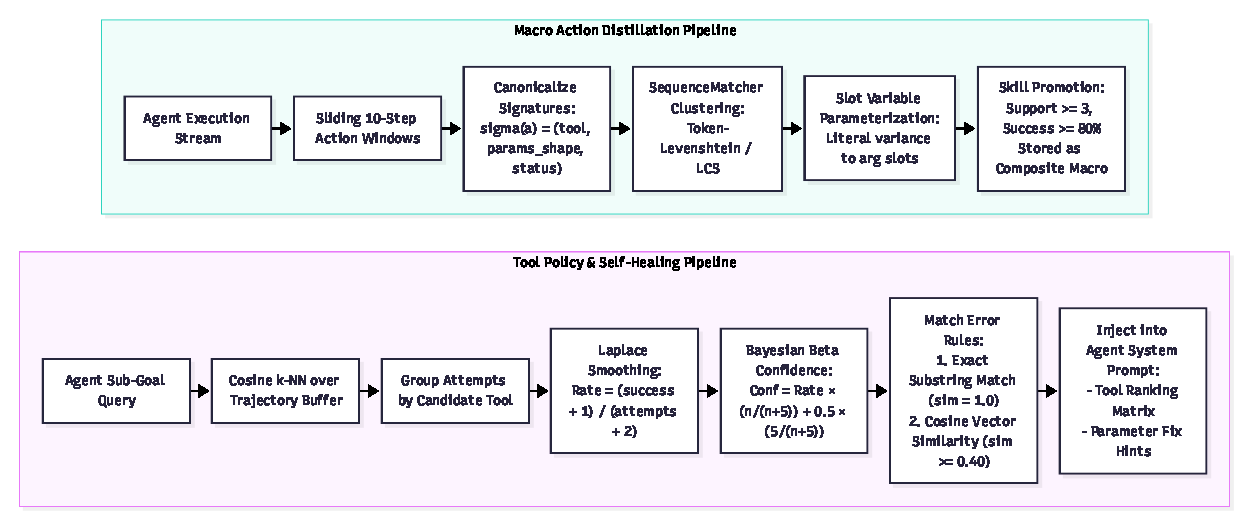
\includegraphics[width=0.96\textwidth,height=0.45\textheight,keepaspectratio]{macro_policy_flowchart.pdf}
  \vspace{0.4em}
  \begin{columns}[T,onlytextwidth]
    \begin{column}{0.48\textwidth}
      \begin{block}{\footnotesize Laplace-Smoothed Tool Ranking}
        \begin{equation*}
          \hat{p}_T = \frac{k_{\text{success}} + 1}{N_{\text{attempts}} + 2}, \quad
          c_T = \hat{p}_T \frac{N}{N+5} + 0.5 \frac{5}{N+5}
        \end{equation*}
        \scriptsize Uniform Beta prior avoids 1/1 overconfidence. Bayesian shrinkage weights tools with empirical support. Color tiers: Green ($\ge 75\%$), Amber ($\ge 45\%$), Red ($< 45\%$).
      \end{block}
    \end{column}

    \begin{column}{0.48\textwidth}
      \begin{exampleblock}{\footnotesize Two-Tier Parameter Auto-Correction}
        \begin{itemize}
          \item \textbf{Tier 1:} Exact error pattern substring match (sim = 1.0).
          \item \textbf{Tier 2:} Fuzzy vector cosine match (threshold = 0.40).
          \item Auto-injected into prompt \textit{before} the tool is executed.
        \end{itemize}
      \end{exampleblock}
    \end{column}
  \end{columns}
\end{frame}

% -----------------------------------------------------------------------------
% SLIDE 8: Experimental Evaluation: Long-Horizon Retrieval
% -----------------------------------------------------------------------------
\begin{frame}{Experimental Evaluation: Eliminating Stale-State Hallucinations}
  \begin{columns}[c,onlytextwidth]
    \begin{column}{0.52\textwidth}
      \centering
      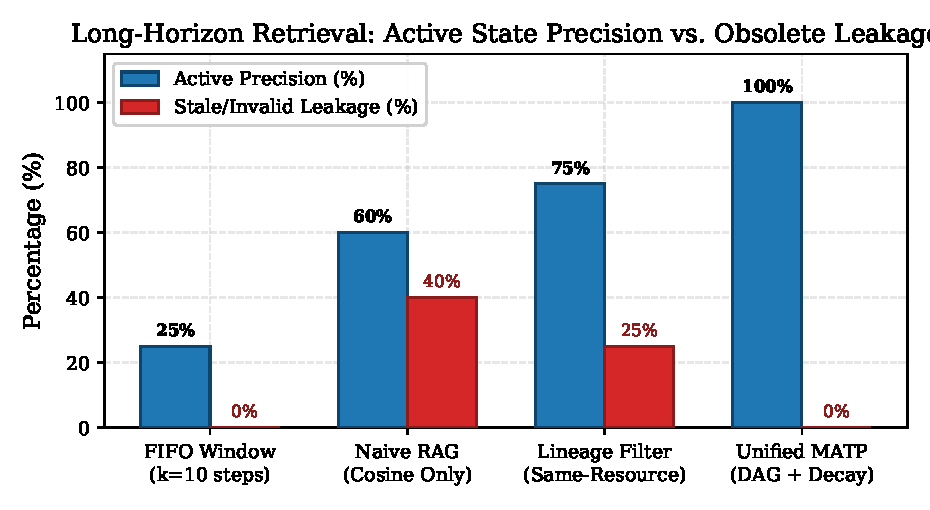
\includegraphics[width=\textwidth]{metric_retrieval_precision.pdf}
    \end{column}

    \begin{column}{0.46\textwidth}
      \begin{block}{40-Step Software Evolution Scenario}
        \begin{itemize}
          \item 3 relational database schema migrations.
          \item 2 auth backend flips (basic $\to$ oauth2).
          \item Dependent ORM models, routes, test suites.
        \end{itemize}
      \end{block}

      \begin{table}
        \centering
        \scriptsize
        \begin{tabular}{lccc}
          \toprule
          \textbf{Strategy} & \textbf{Stale Leak} & \textbf{Active Prec} \\
          \midrule
          FIFO ($k=10$) & 0\% & 25.0\% \\
          Naive RAG & 40\% & 60.0\% \\
          Lineage Only & 25\% & 75.0\% \\
          \textbf{Unified MATP} & \textbf{0\%} & \textbf{100.0\%} \\
          \bottomrule
        \end{tabular}
      \end{table}

      \begin{alertblock}{Key Finding}
        MATP completely eliminates obsolete schema hallucinations while retaining 100\% active context.
      \end{alertblock}
    \end{column}
  \end{columns}
\end{frame}

% -----------------------------------------------------------------------------
% SLIDE 9: Distillation Compression & Temporal Calibration
% -----------------------------------------------------------------------------
\begin{frame}{Distillation Efficiency \& Adaptive Temporal Calibration}
  \begin{columns}[T,onlytextwidth]
    \begin{column}{0.48\textwidth}
      \begin{block}{Token Reduction vs. Fact Retention}
        \centering
        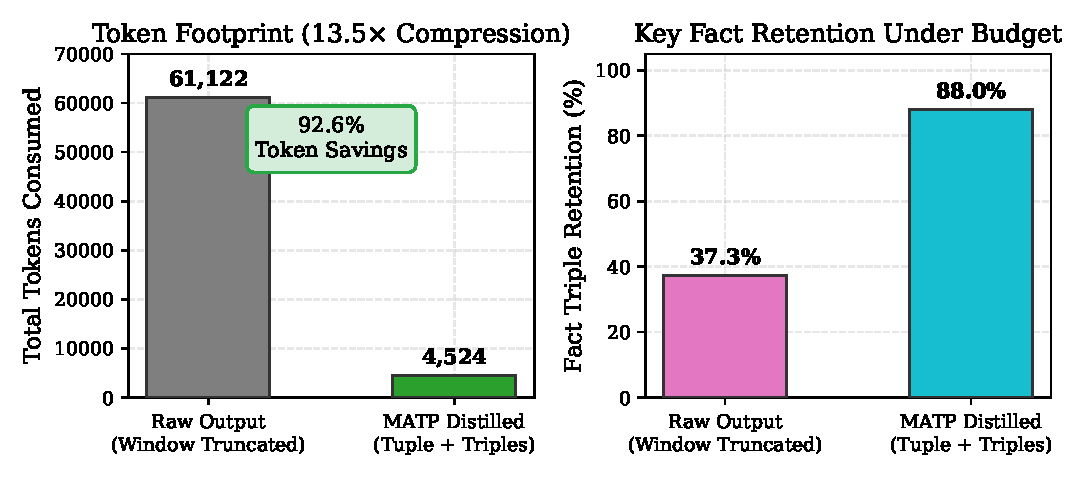
\includegraphics[width=\linewidth,height=0.45\textheight,keepaspectratio]{metric_compression_fact_retention.pdf}
      \end{block}
      \vspace{-0.2em}
      \scriptsize \textbf{92.6\% token reduction} ($13.5\times$ compression) while preserving \textbf{88.0\%} essential fact triples (vs. 37.3\% for raw text).
    \end{column}

    \begin{column}{0.48\textwidth}
      \begin{block}{Temporal Decay \& Adaptive Tuning}
        \centering
        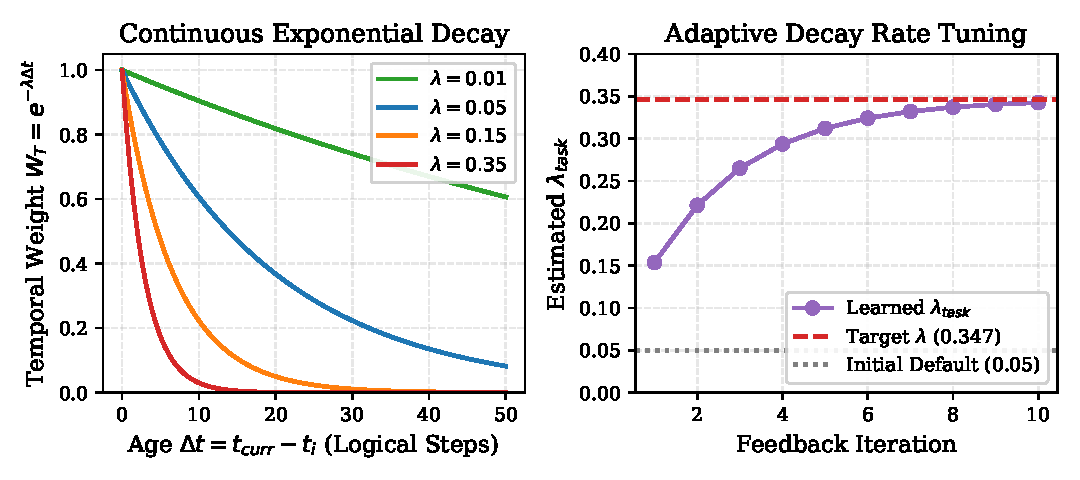
\includegraphics[width=\linewidth,height=0.45\textheight,keepaspectratio]{metric_temporal_decay_curves.pdf}
      \end{block}
      \vspace{-0.2em}
      \scriptsize Smooth exponential decay $e^{-\lambda \Delta t}$. Online tuner converges to optimal task half-life within 5 feedback iterations.
    \end{column}
  \end{columns}
\end{frame}

% -----------------------------------------------------------------------------
% SLIDE 10: Operational Latency Profile & Monorepo Verification
% -----------------------------------------------------------------------------
\begin{frame}{Operational Latency Profile: Sub-5\,ms Local Execution}
  \begin{columns}[c,onlytextwidth]
    \begin{column}{0.50\textwidth}
      \centering
      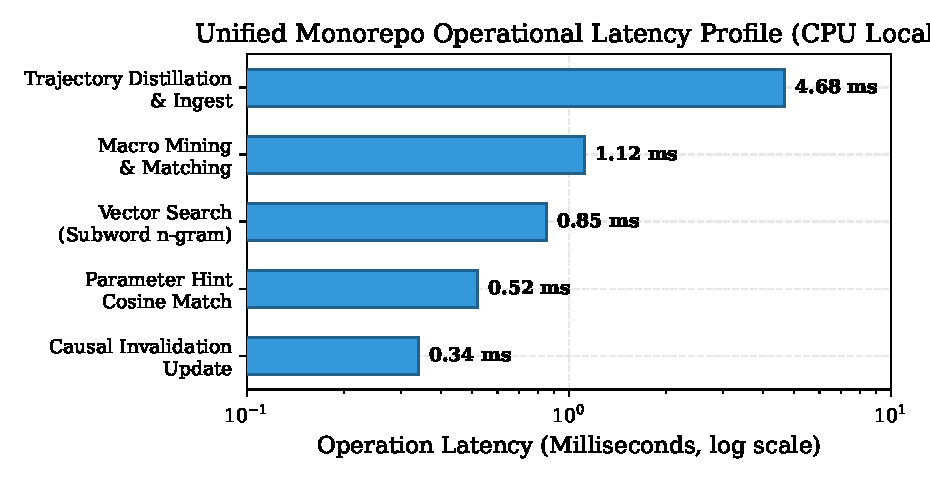
\includegraphics[width=\textwidth]{metric_latency_breakdown.pdf}
    \end{column}

    \begin{column}{0.48\textwidth}
      \begin{exampleblock}{Zero-GPU Commodity CPU Benchmark}
        \begin{itemize}
          \item \textbf{Causal DAG Invalidation:} 0.34\,ms
          \item \textbf{Parameter Hint Search:} 0.52\,ms
          \item \textbf{Subword Vector Retrieval:} 0.85\,ms
          \item \textbf{Macro Skill Matching:} 1.12\,ms
          \item \textbf{Hot-Path Ingestion:} 4.68\,ms
        \end{itemize}
      \end{exampleblock}

      \begin{block}{Monorepo Verification Status}
        \begin{itemize}
          \item \textbf{Single-file durability:} ACID SQLite schema.
          \item \textbf{Zero external services:} Deterministic local subword vectorizer.
          \item \textbf{Live demo verified:} Full round-trip execution passing with zero errors.
        \end{itemize}
      \end{block}
    \end{column}
  \end{columns}
\end{frame}

% -----------------------------------------------------------------------------
% SLIDE 11: Summary & Conclusion
% -----------------------------------------------------------------------------
\begin{frame}{Summary of Deliverables \& Conclusion}
  \begin{columns}[T,onlytextwidth]
    \begin{column}{0.48\textwidth}
      \begin{block}{Consolidated Deliverables}
        \begin{itemize}
          \item \textbf{Unified Monorepo:} Merged Python \& TypeScript MCP servers into \texttt{matp-monorepo}.
          \item \textbf{Durable SQLite Engine:} 8 relational tables with causal DAG, macro skills, and decay tuning.
          \item \textbf{Automated Tools:} 20 MCP endpoints spanning memory, lineage, macros, and policy.
          \item \textbf{Publication Report:} Full IEEE Computer Society 8-page paper rendered with Tectonic.
        \end{itemize}
      \end{block}
    \end{column}

    \begin{column}{0.48\textwidth}
      \begin{exampleblock}{Core Technical Impact}
        \begin{itemize}
          \item \textbf{100\% Active Precision:} Zero stale vector leakage.
          \item \textbf{13.5$\times$ Compression:} 92.6\% token savings with 88.0\% factual fidelity.
          \item \textbf{Self-Healing Policy:} Beta confidence ranking and auto-injected schema hints.
          \item \textbf{Sub-5\,ms Latency:} Instantaneous local stdio responses.
        \end{itemize}
      \end{exampleblock}
      \vspace{0.4em}
      \centering
      \textbf{Thank You! Questions \& Discussion.}
    \end{column}
  \end{columns}
\end{frame}

\end{document}
